\begin{figure}[htpb]
    \centering
    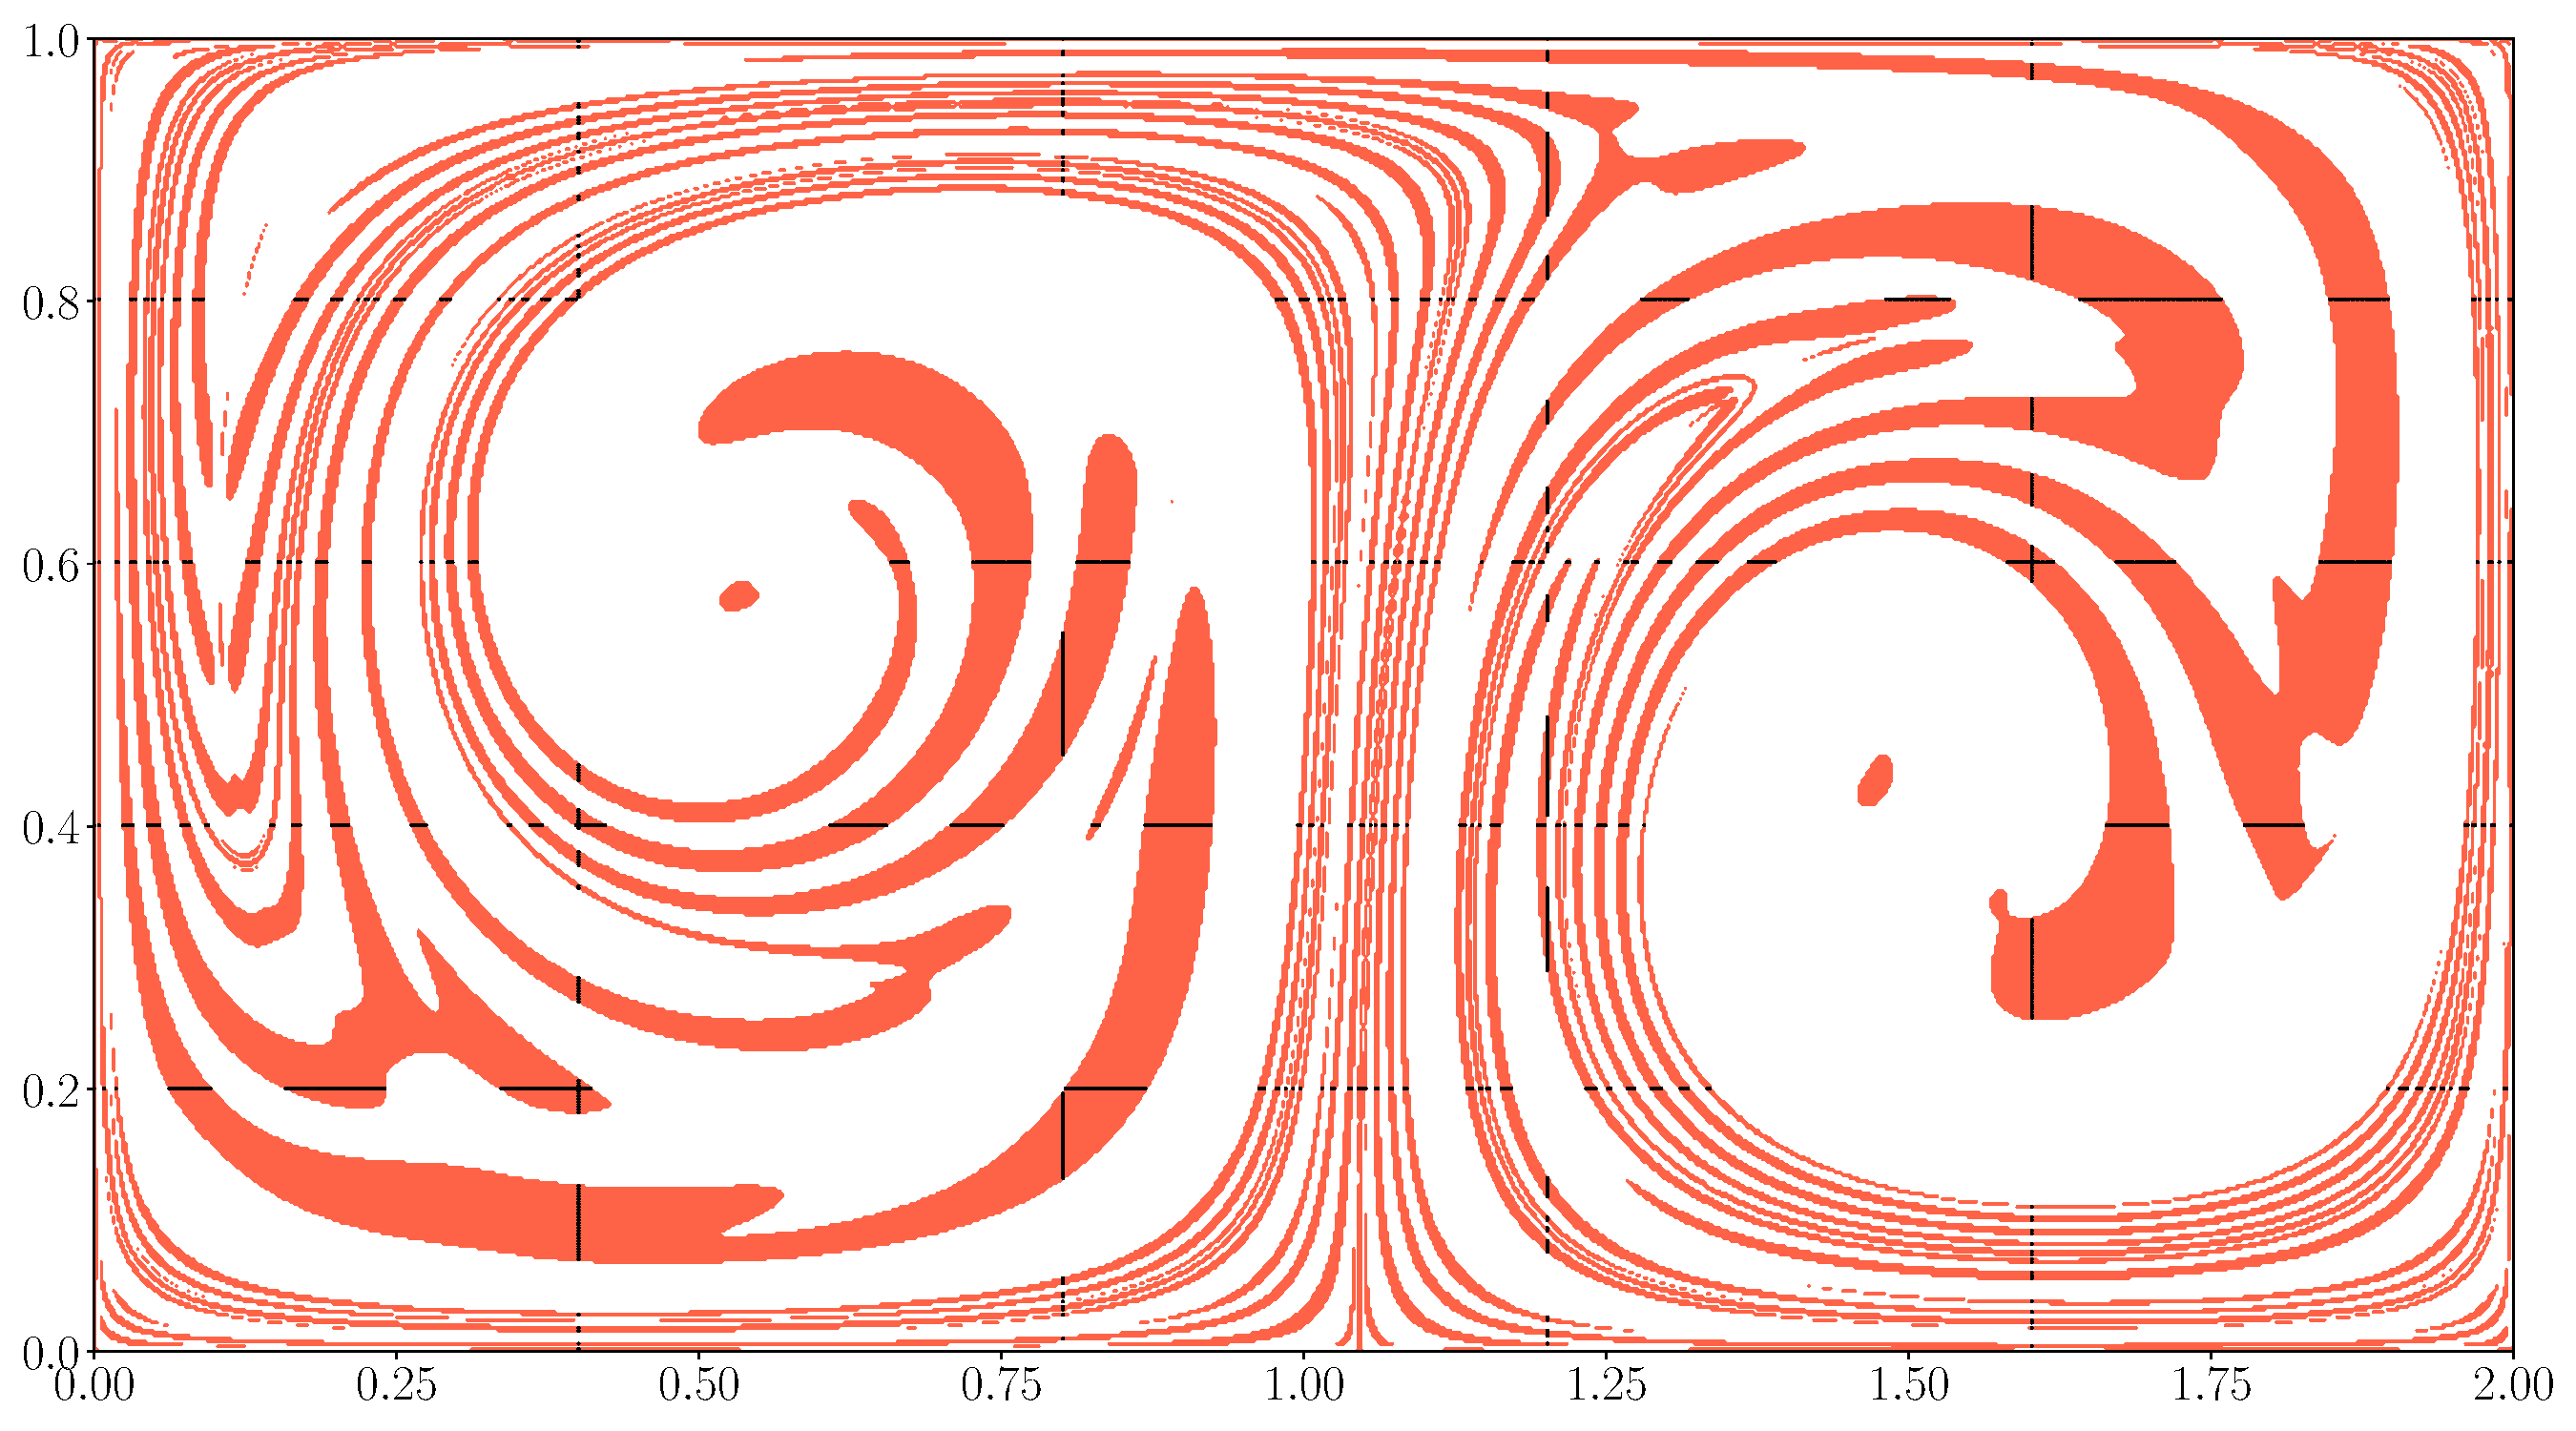
\includegraphics[width=0.9\linewidth,keepaspectratio]{figures/u0_domain.pdf}
    \caption[The set $\mathcal{U}_{0}$ for the double gyre system]{The set
    $\mathcal{U}_{0}$ for the double gyre system, given by equations
    \eqref{eq:doublegyre} and \eqref{eq:doublegyreparams}, is shown in red. Its
    itersection with a set of four horizontal and four vertical, equidistant
    lines is shown in black. The latter was used as the set of strain initial
    conditions, in order to eliminate redundant computations of strainlines
    within $\mathcal{U}_{0}$.}
    \label{fig:u0_domain}
\end{figure}
